\section{Shock wave simulation}
We studied the influence of fractions of heavy ions on the shock wave, in particular, the spectrum of particles and the shape of the shock wave. We present results of two simulations with different compositions of the plasma : pure protons and electrons in the first case and with the admixture of alpha particles in the second case. Initially the homogeneous flux is  moving from the right free boundary to the left. On the left side there is a reflecting super-conducting wall, which causes formation of shock wave. Simulations are one-dimensional and have following parameters: initial velocity $v = 0.2c$, number densities $n_e = 10^{-4} \rm{cm}^{-3}$, $n_p = 10^{-4} \rm{cm}^{-3}$ in the first simulation and $n_e = 10^{-4} \rm{cm}^{-3}$, $n_p = 0.6\cdot10^{-4} \rm{cm}^{-3}$, $n_\alpha = 0.2\cdot10^{-4} \rm{cm}^{-3}$ in the second, temperature $5\cdot10^8 \rm{K}$, magnetic field $B_\parallel = 10^{-4} \rm{G}, B_\perp= 0.7\cdot10^{-4} \rm{G}$, the full size of the box $L = 1\cdot10^{12} \rm{cm}$, the number of cells $N=2\cdot10^4$. Electron mass is reduced to $m_e = \frac{m_p}{20}$. The full time of simulation is $T = 2000 {\omega_p}^{-1}$.
\begin{figure}[h!]
	\centering
	\begin{minipage}{0.49\textwidth}
		\centering
		%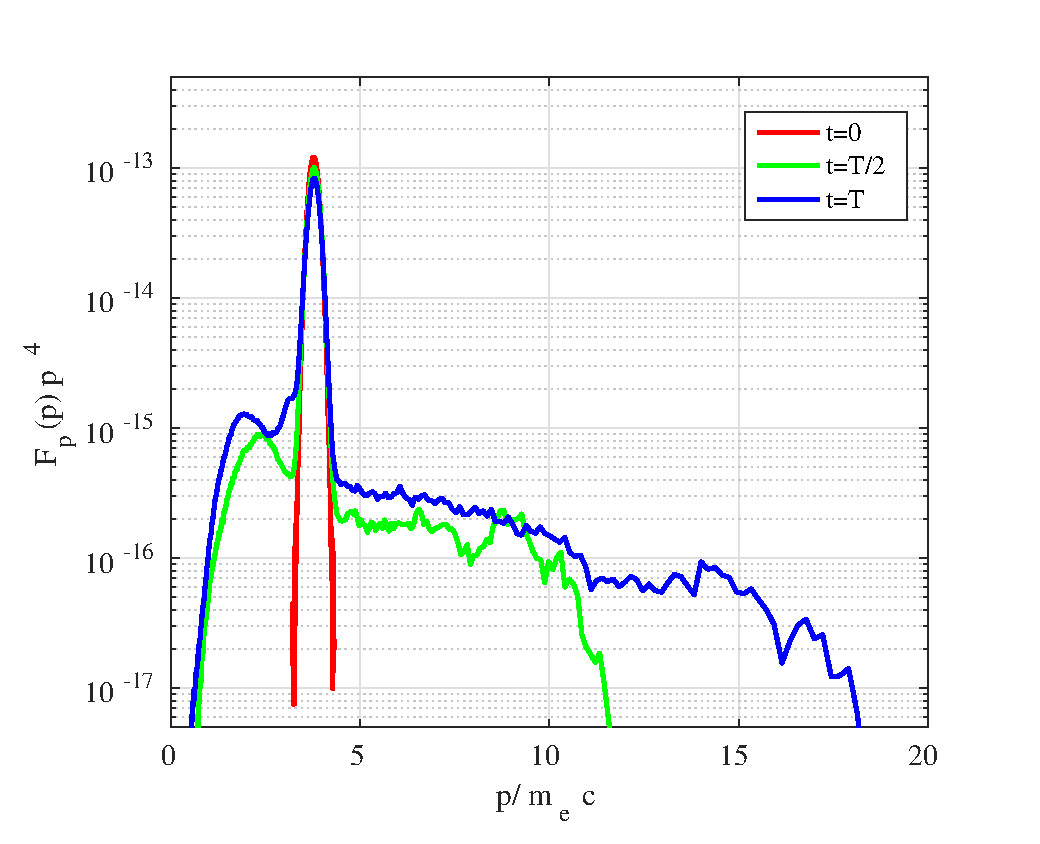
\includegraphics[width=0.98\textwidth]{fig/protons.eps} 
		\caption{Distribution of protons in the simulation without alpha particles.}
		\label{protons}
	\end{minipage}\hfill
	\begin{minipage}{0.49\textwidth}
		\centering
		%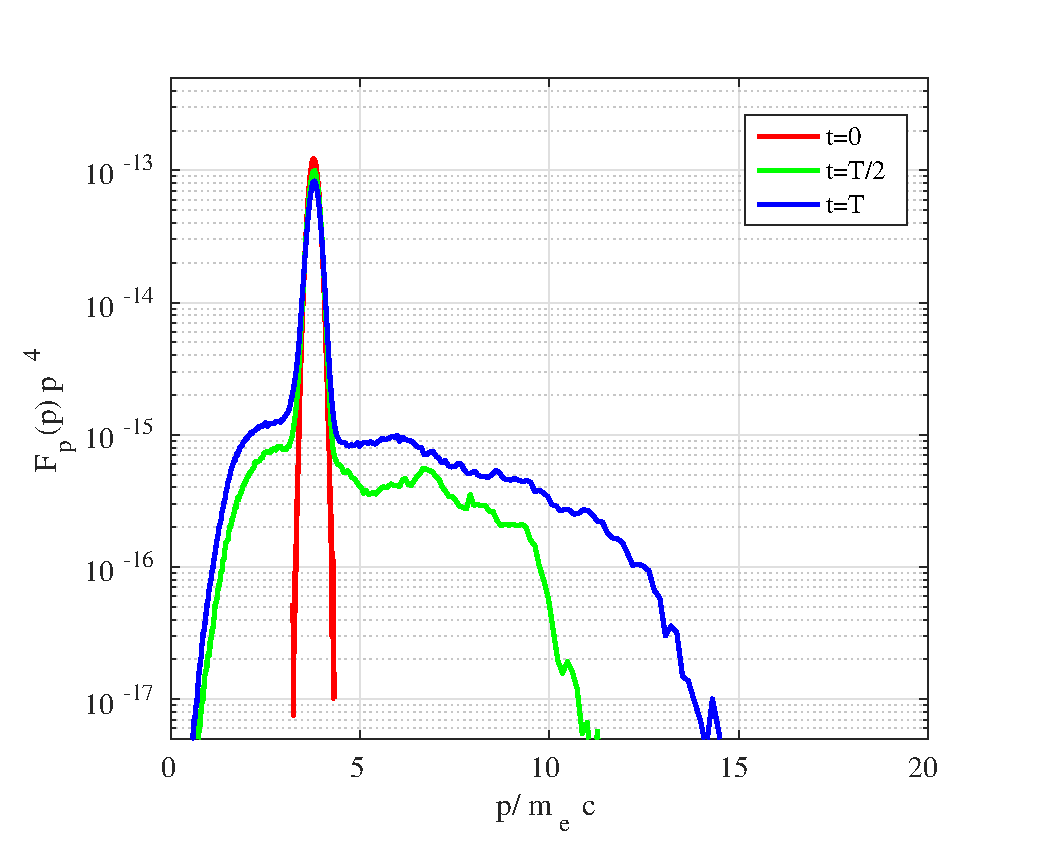
\includegraphics[width=0.98\textwidth]{fig/protons_with_He.eps} 
		\caption{Distribution of protons in the simulation with alpha particles.}
		\label{protons_with_alpha}
	\end{minipage}
\end{figure}
\begin{figure}[h!]
	\centering
	\begin{minipage}{0.49\textwidth}
		\centering
		%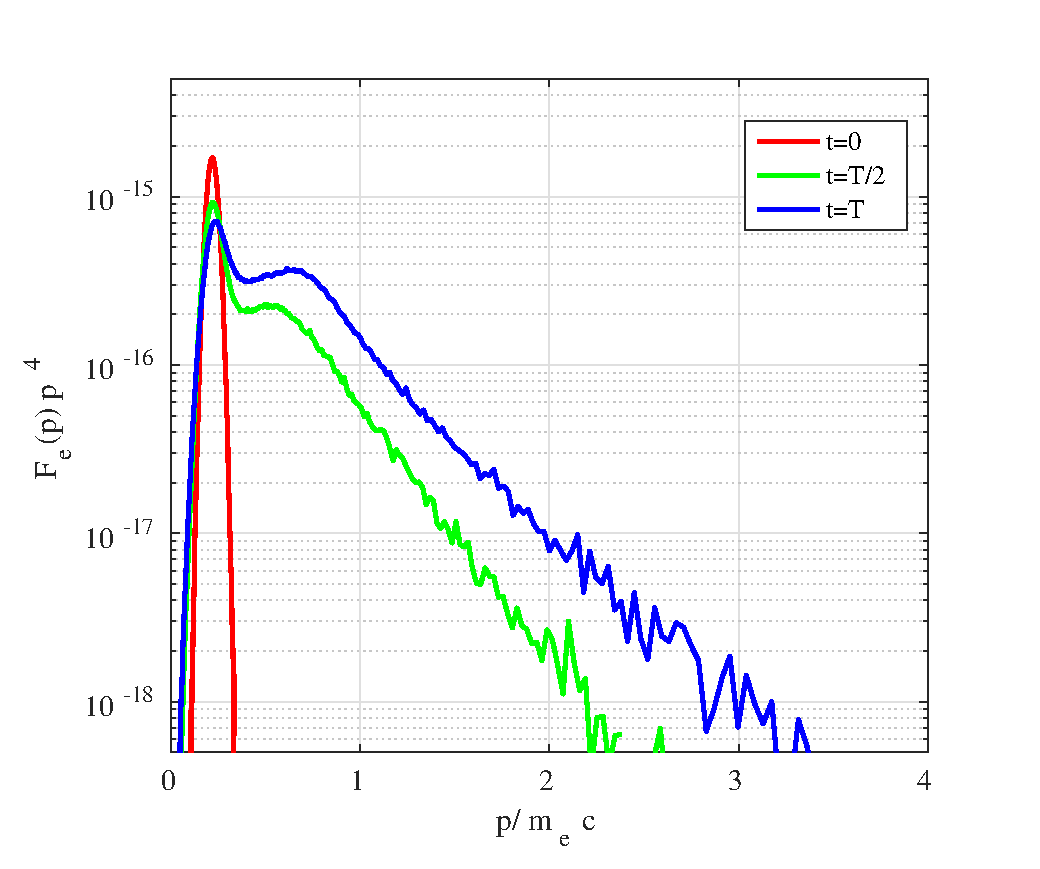
\includegraphics[width=0.98\textwidth]{fig/electrons.eps} 
		\caption{Distribution of electrons in the simulation without alpha particles.}
		\label{electrons}
	\end{minipage}\hfill
	\begin{minipage}{0.49\textwidth}
		\centering
		%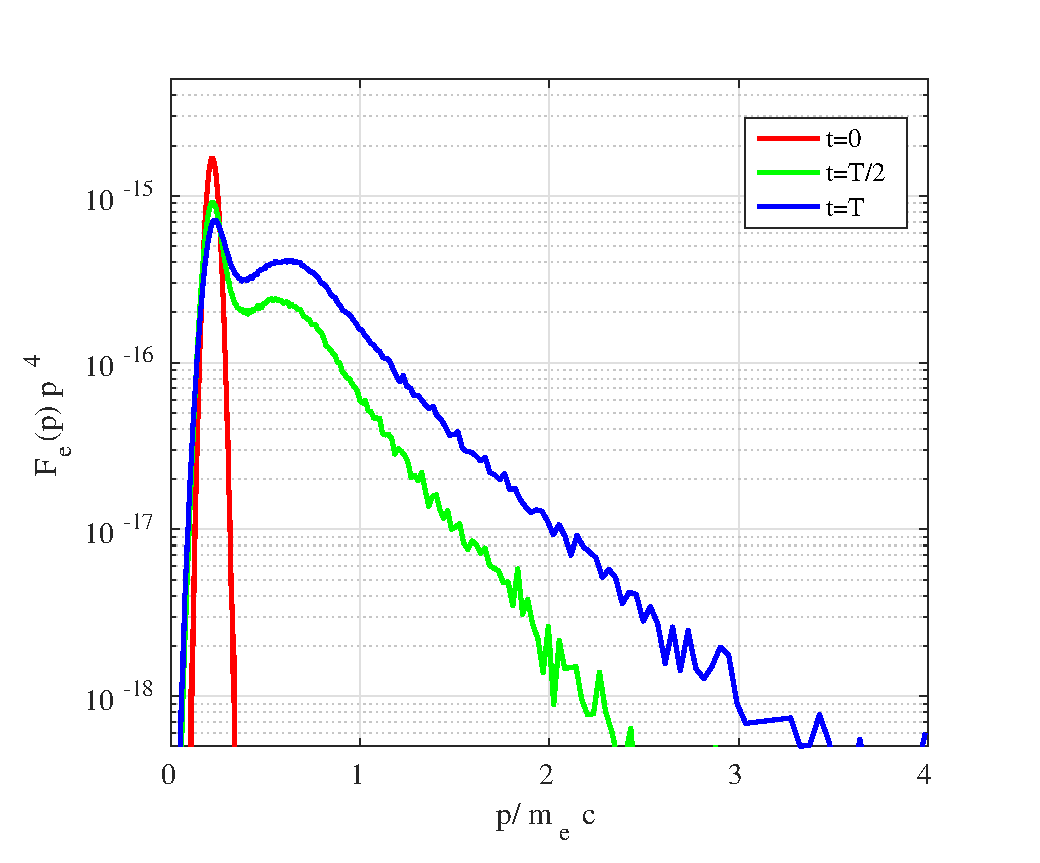
\includegraphics[width=0.98\textwidth]{fig/electrons_with_He.eps} 
		\caption{Distribution of electrons in the simulation with alpha particles.}
		\label{electrons_with_alpha}
	\end{minipage}
\end{figure}

The results presented in Figures \ref{protons}-\ref{electrons_with_alpha} show that the values of $F(p)p^4$ for high energies are much greater for protons, than for electrons in both simulations. Also electrons need much more time to be accelerated and to form spectrum $\propto p^{-4}$. It means that protons are injected into the acceleration process more efficiently, and it is consistent with the work of Park et al. {\cite{Park2015}}. Also we have shown that minority of heavy ions increases the spectrum of protons and do not have influence on the spectrum of electrons. It can be explained by the fact, that heavy ions form the large scale turbulence and protons can efficiently scatter on this turbulence. Otherwise for electrons turbulence produced by protons is already enough large-scale  and the influence of heavy ions is neglectable. 
